\section{Casi d'uso}
\subsection{Attori dei casi d'uso}
	
	\subsubsection{Attori primari}
		\begin{figure}[h]
			\centering
			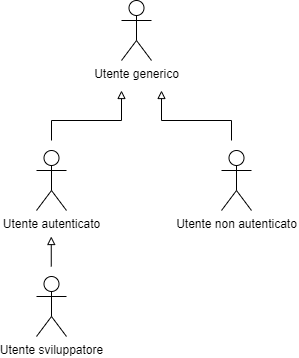
\includegraphics[scale=0.5]{./res/img/gerarchia.png}
			\caption {Gerarchia degli attori}
		\end{figure}
		\begin{description}[style=nextline]
			\item[\textbf{Utente generico}]
				Si riferisce ad un utente generico che ha avviato l'applicativo. 
			\item[\textbf{Utente non autenticato}]
				Si riferisce ad un utente generico che non ha ancora effettuato l'autenticazione all'interno della rete Ethereum. 
			\item[\textbf{Utente autenticato}]
				Si riferisce ad un utente generico che si è autenticato nel sistema tramite il comando di login. Ciò implica che sia in possesso di una chiave o una frase mnemonica valida all'interno della rete Ethereum. 
			\item[\textbf{Utente sviuppatore}] 
				Si riferisce ad un utente autenticato che ha svolto il deploy di almeno una sua funzione. 
		\end{description}
	
	\subsubsection{Attori secondari}
		\begin{description}[style=nextline]
			\item[\textbf{Ethereum network}]
				Piattaforma decentralizzata utilizzata per la gestione dell'autenticazione, dei pagamenti e della comunicazione tra i vari moduli della piattaforma \textit{Etherless}. 
		\end{description}
	\pagebreak
\subsection{Elenco dei casi d'uso}
In questa sezione vengono elencati tutti i casi d'uso individuati. Ogni caso d'uso rappresenta uno scenario per uno o più attori, ed è descritto tramite degli appositi diagrammi dei casi d'uso. 

\subsubsection*{Operazioni utenti}
Di seguito sono riportati tutti i casi d'uso aventi come attore primario l'utente generico, l'utente non autenticato o l'utente autenticato. 

\subsubsection{Visualizzazione guida introduttiva}
	\begin{figure}[h]
		\centering
		
\includegraphics[scale=0.15]{./res/img/UC1-GuidaIntro.png}
		\caption {UC1 - Visualizzazione guida introduttiva}
	\end{figure}
	\begin{itemize}
		\item \textbf{Attori primari:} utente generico
		\item \textbf{Descrizione:} l'utente visualizza una guida contenente una breve spiegazione per ogni comando disponibile in \textit{Etheress-cli}. Tale guida ha lo scopo di aiutare l'utente a procedere nell'utilizzo dell'applicativo; 
		\item \textbf{Scenario principale:} l'utente avvia l'applicativo e visualizza la guida; 
		\item \textbf{Precondizione:} l'utente avvia l'applicativo tramite il comando "etherless-init" e quest'ultimo si apre correttamente; 
		\item \textbf{Postcondizione:} il sistema fornisce all'utente tutte le informazioni necessarie per procedere con l'utilizzo dell'applicativo. 
	\end{itemize}
\subsubsection{Registrazione} 
	\begin{figure}[h]
	\centering
	
\includegraphics[scale=0.15]{./res/img/UC1-GuidaIntro.png}
	\caption {UC1 - Visualizzazione guida introduttiva}
\end{figure}
\begin{itemize}
	\item \textbf{Attori primari:}
	\item \textbf{Descrizione:} 
	\item \textbf{Scenario principale:} 
	\item \textbf{Precondizione:} 
	\item \textbf{Postcondizione:} 
\end{itemize}
% \subsubsection{Visualizzazione guida introduttiva}
	\begin{figure}[h]
		\centering
		
\includegraphics[scale=0.15]{./res/img/UC1-GuidaIntro.png}
		\caption {UC1 - Visualizzazione guida introduttiva}
	\end{figure}
	\begin{itemize}
		\item \textbf{Attori primari:} utente generico
		\item \textbf{Descrizione:} l'utente visualizza una guida contenente una breve spiegazione per ogni comando disponibile in \textit{Etheress-cli}. Tale guida ha lo scopo di aiutare l'utente a procedere nell'utilizzo dell'applicativo; 
		\item \textbf{Scenario principale:} l'utente avvia l'applicativo e visualizza la guida; 
		\item \textbf{Precondizione:} l'utente avvia l'applicativo tramite il comando "etherless-init" e quest'ultimo si apre correttamente; 
		\item \textbf{Postcondizione:} il sistema fornisce all'utente tutte le informazioni necessarie per procedere con l'utilizzo dell'applicativo. 
	\end{itemize}
% \subsubsection{Visualizzazione guida introduttiva}
	\begin{figure}[h]
		\centering
		
\includegraphics[scale=0.15]{./res/img/UC1-GuidaIntro.png}
		\caption {UC1 - Visualizzazione guida introduttiva}
	\end{figure}
	\begin{itemize}
		\item \textbf{Attori primari:} utente generico
		\item \textbf{Descrizione:} l'utente visualizza una guida contenente una breve spiegazione per ogni comando disponibile in \textit{Etheress-cli}. Tale guida ha lo scopo di aiutare l'utente a procedere nell'utilizzo dell'applicativo; 
		\item \textbf{Scenario principale:} l'utente avvia l'applicativo e visualizza la guida; 
		\item \textbf{Precondizione:} l'utente avvia l'applicativo tramite il comando "etherless-init" e quest'ultimo si apre correttamente; 
		\item \textbf{Postcondizione:} il sistema fornisce all'utente tutte le informazioni necessarie per procedere con l'utilizzo dell'applicativo. 
	\end{itemize}
% \subsubsection{Visualizzazione guida introduttiva}
	\begin{figure}[h]
		\centering
		
\includegraphics[scale=0.15]{./res/img/UC1-GuidaIntro.png}
		\caption {UC1 - Visualizzazione guida introduttiva}
	\end{figure}
	\begin{itemize}
		\item \textbf{Attori primari:} utente generico
		\item \textbf{Descrizione:} l'utente visualizza una guida contenente una breve spiegazione per ogni comando disponibile in \textit{Etheress-cli}. Tale guida ha lo scopo di aiutare l'utente a procedere nell'utilizzo dell'applicativo; 
		\item \textbf{Scenario principale:} l'utente avvia l'applicativo e visualizza la guida; 
		\item \textbf{Precondizione:} l'utente avvia l'applicativo tramite il comando "etherless-init" e quest'ultimo si apre correttamente; 
		\item \textbf{Postcondizione:} il sistema fornisce all'utente tutte le informazioni necessarie per procedere con l'utilizzo dell'applicativo. 
	\end{itemize}
% \subsubsection{Visualizzazione guida introduttiva}
	\begin{figure}[h]
		\centering
		
\includegraphics[scale=0.15]{./res/img/UC1-GuidaIntro.png}
		\caption {UC1 - Visualizzazione guida introduttiva}
	\end{figure}
	\begin{itemize}
		\item \textbf{Attori primari:} utente generico
		\item \textbf{Descrizione:} l'utente visualizza una guida contenente una breve spiegazione per ogni comando disponibile in \textit{Etheress-cli}. Tale guida ha lo scopo di aiutare l'utente a procedere nell'utilizzo dell'applicativo; 
		\item \textbf{Scenario principale:} l'utente avvia l'applicativo e visualizza la guida; 
		\item \textbf{Precondizione:} l'utente avvia l'applicativo tramite il comando "etherless-init" e quest'ultimo si apre correttamente; 
		\item \textbf{Postcondizione:} il sistema fornisce all'utente tutte le informazioni necessarie per procedere con l'utilizzo dell'applicativo. 
	\end{itemize}

\subsubsection*{Operazioni sviluppatori}
Di seguito sono riportati tutti i casi d'uso aventi come attore primario l'utente sviluppatore.

% \subsubsection{Visualizzazione guida introduttiva}
	\begin{figure}[h]
		\centering
		
\includegraphics[scale=0.15]{./res/img/UC1-GuidaIntro.png}
		\caption {UC1 - Visualizzazione guida introduttiva}
	\end{figure}
	\begin{itemize}
		\item \textbf{Attori primari:} utente generico
		\item \textbf{Descrizione:} l'utente visualizza una guida contenente una breve spiegazione per ogni comando disponibile in \textit{Etheress-cli}. Tale guida ha lo scopo di aiutare l'utente a procedere nell'utilizzo dell'applicativo; 
		\item \textbf{Scenario principale:} l'utente avvia l'applicativo e visualizza la guida; 
		\item \textbf{Precondizione:} l'utente avvia l'applicativo tramite il comando "etherless-init" e quest'ultimo si apre correttamente; 
		\item \textbf{Postcondizione:} il sistema fornisce all'utente tutte le informazioni necessarie per procedere con l'utilizzo dell'applicativo. 
	\end{itemize}
% \subsubsection{Visualizzazione guida introduttiva}
	\begin{figure}[h]
		\centering
		
\includegraphics[scale=0.15]{./res/img/UC1-GuidaIntro.png}
		\caption {UC1 - Visualizzazione guida introduttiva}
	\end{figure}
	\begin{itemize}
		\item \textbf{Attori primari:} utente generico
		\item \textbf{Descrizione:} l'utente visualizza una guida contenente una breve spiegazione per ogni comando disponibile in \textit{Etheress-cli}. Tale guida ha lo scopo di aiutare l'utente a procedere nell'utilizzo dell'applicativo; 
		\item \textbf{Scenario principale:} l'utente avvia l'applicativo e visualizza la guida; 
		\item \textbf{Precondizione:} l'utente avvia l'applicativo tramite il comando "etherless-init" e quest'ultimo si apre correttamente; 
		\item \textbf{Postcondizione:} il sistema fornisce all'utente tutte le informazioni necessarie per procedere con l'utilizzo dell'applicativo. 
	\end{itemize}
% \subsubsection{Visualizzazione guida introduttiva}
	\begin{figure}[h]
		\centering
		
\includegraphics[scale=0.15]{./res/img/UC1-GuidaIntro.png}
		\caption {UC1 - Visualizzazione guida introduttiva}
	\end{figure}
	\begin{itemize}
		\item \textbf{Attori primari:} utente generico
		\item \textbf{Descrizione:} l'utente visualizza una guida contenente una breve spiegazione per ogni comando disponibile in \textit{Etheress-cli}. Tale guida ha lo scopo di aiutare l'utente a procedere nell'utilizzo dell'applicativo; 
		\item \textbf{Scenario principale:} l'utente avvia l'applicativo e visualizza la guida; 
		\item \textbf{Precondizione:} l'utente avvia l'applicativo tramite il comando "etherless-init" e quest'ultimo si apre correttamente; 
		\item \textbf{Postcondizione:} il sistema fornisce all'utente tutte le informazioni necessarie per procedere con l'utilizzo dell'applicativo. 
	\end{itemize}
% \subsubsection{Visualizzazione guida introduttiva}
	\begin{figure}[h]
		\centering
		
\includegraphics[scale=0.15]{./res/img/UC1-GuidaIntro.png}
		\caption {UC1 - Visualizzazione guida introduttiva}
	\end{figure}
	\begin{itemize}
		\item \textbf{Attori primari:} utente generico
		\item \textbf{Descrizione:} l'utente visualizza una guida contenente una breve spiegazione per ogni comando disponibile in \textit{Etheress-cli}. Tale guida ha lo scopo di aiutare l'utente a procedere nell'utilizzo dell'applicativo; 
		\item \textbf{Scenario principale:} l'utente avvia l'applicativo e visualizza la guida; 
		\item \textbf{Precondizione:} l'utente avvia l'applicativo tramite il comando "etherless-init" e quest'ultimo si apre correttamente; 
		\item \textbf{Postcondizione:} il sistema fornisce all'utente tutte le informazioni necessarie per procedere con l'utilizzo dell'applicativo. 
	\end{itemize}
% \subsubsection{Visualizzazione guida introduttiva}
	\begin{figure}[h]
		\centering
		
\includegraphics[scale=0.15]{./res/img/UC1-GuidaIntro.png}
		\caption {UC1 - Visualizzazione guida introduttiva}
	\end{figure}
	\begin{itemize}
		\item \textbf{Attori primari:} utente generico
		\item \textbf{Descrizione:} l'utente visualizza una guida contenente una breve spiegazione per ogni comando disponibile in \textit{Etheress-cli}. Tale guida ha lo scopo di aiutare l'utente a procedere nell'utilizzo dell'applicativo; 
		\item \textbf{Scenario principale:} l'utente avvia l'applicativo e visualizza la guida; 
		\item \textbf{Precondizione:} l'utente avvia l'applicativo tramite il comando "etherless-init" e quest'ultimo si apre correttamente; 
		\item \textbf{Postcondizione:} il sistema fornisce all'utente tutte le informazioni necessarie per procedere con l'utilizzo dell'applicativo. 
	\end{itemize}
% \subsubsection{Visualizzazione guida introduttiva}
	\begin{figure}[h]
		\centering
		
\includegraphics[scale=0.15]{./res/img/UC1-GuidaIntro.png}
		\caption {UC1 - Visualizzazione guida introduttiva}
	\end{figure}
	\begin{itemize}
		\item \textbf{Attori primari:} utente generico
		\item \textbf{Descrizione:} l'utente visualizza una guida contenente una breve spiegazione per ogni comando disponibile in \textit{Etheress-cli}. Tale guida ha lo scopo di aiutare l'utente a procedere nell'utilizzo dell'applicativo; 
		\item \textbf{Scenario principale:} l'utente avvia l'applicativo e visualizza la guida; 
		\item \textbf{Precondizione:} l'utente avvia l'applicativo tramite il comando "etherless-init" e quest'ultimo si apre correttamente; 
		\item \textbf{Postcondizione:} il sistema fornisce all'utente tutte le informazioni necessarie per procedere con l'utilizzo dell'applicativo. 
	\end{itemize}
